\section{Lambda-Kalkül}
\subsection{Untypisiertes Lambdakalkül}
\textbf{linksassoziativ}
\begin{defi}[$\alpha$-Äquiv]
	Terme $t_1$,  $t_2$ $\alpha$-äquivalent $\Leftrightarrow$ $t1$ durch Ersetzen der gebunden Variablen in $t2$ überführbar
\end{defi}
Beispiel: $\lambda y.y \stackrel{\alpha}{=} \lambda x.x$

\subsubsection{Ausführungsreihenfolge}

\begin{defi}[Normalenreihenfolge]
	Linkest-äußersten Term zuerst
\end{defi}
Beispiel 1:\\
$$(\lambda x.x)((\lambda x.x) (\lambda z. (\lambda x.x) z))$$
$$ \Rightarrow ((\lambda x.x) (\lambda z. (\lambda x.x) z))$$
$$ \Rightarrow (\lambda z. (\lambda x.x) z)$$
$$ \Rightarrow (\lambda z. z)$$
Beispiel 2:\\
$$(\lambda y. (\lambda x. y (\lambda z.z) x)) ((\lambda x.x) (\lambda y.y))$$
$$\Rightarrow \lambda x. ((\lambda x1.x1) (\lambda y.y)) (\lambda z.z) x $$
$$\Rightarrow \lambda x. (\lambda y.y) (\lambda z.z) x$$
$$\Rightarrow \lambda x. (\lambda z.z) x $$
$$\Rightarrow \lambda x. x $$
\begin{defi}[Call-by-name]
		Linkest-äußersten Term zuerst, falls nicht von lambda umgeben
\end{defi}
Beispiel 1:\\
$$(\lambda x.x)((\lambda x.x) (\lambda z. (\lambda x.x) z))$$
$$ \Rightarrow ((\lambda x.x) (\lambda z. (\lambda x.x) z))$$
$$ \Rightarrow (\lambda z. (\lambda x.x) z)$$
Beispiel 2:\\
$$(\lambda y. (\lambda x. y (\lambda z.z) x)) ((\lambda x.x) (\lambda y.y))$$
$$\Rightarrow \lambda x. ((\lambda x1.x1) (\lambda y.y)) (\lambda z.z) x $$
\begin{defi}[Call-by-value]
	Linkest-äußersten Term zuerst, falls nicht von lambda umgeben und dessen Argument ein Wert ist
\end{defi}
Beispiel 1:\\
$$(\lambda x.x)((\lambda x.x) (\lambda z. (\lambda x.x) z))$$
$$ \Rightarrow ((\lambda x.x) (\lambda z. (\lambda x.x) z))$$
$$ \Rightarrow (\lambda z. (\lambda x.x) z)$$
Beispiel 2:\\
$$(\lambda y. (\lambda x. y (\lambda z.z) x)) ((\lambda x.x) (\lambda y.y))$$
$$\Rightarrow \lambda y. (\lambda x. y (\lambda z.z) x)) (\lambda y.y)$$
$$\Rightarrow \lambda x. (\lambda y.y) (\lambda z.z) x))$$

\subsubsection{Rekursion}
Parametrisiere rekursiven aufruf als erstes Argument, verwende Y kombinator\\
Beispiel:\\
$$f = \lambda fak. \lambda n. \medspace (\text{isZero}\medspace n)  \medspace c_1 \medspace (\text{times} \medspace n \medspace (fak (\text{sub}\medspace n \medspace c_1)))$$
$$fak = Y \medspace f$$

\subsection{Typisierung}
\begin{center}
	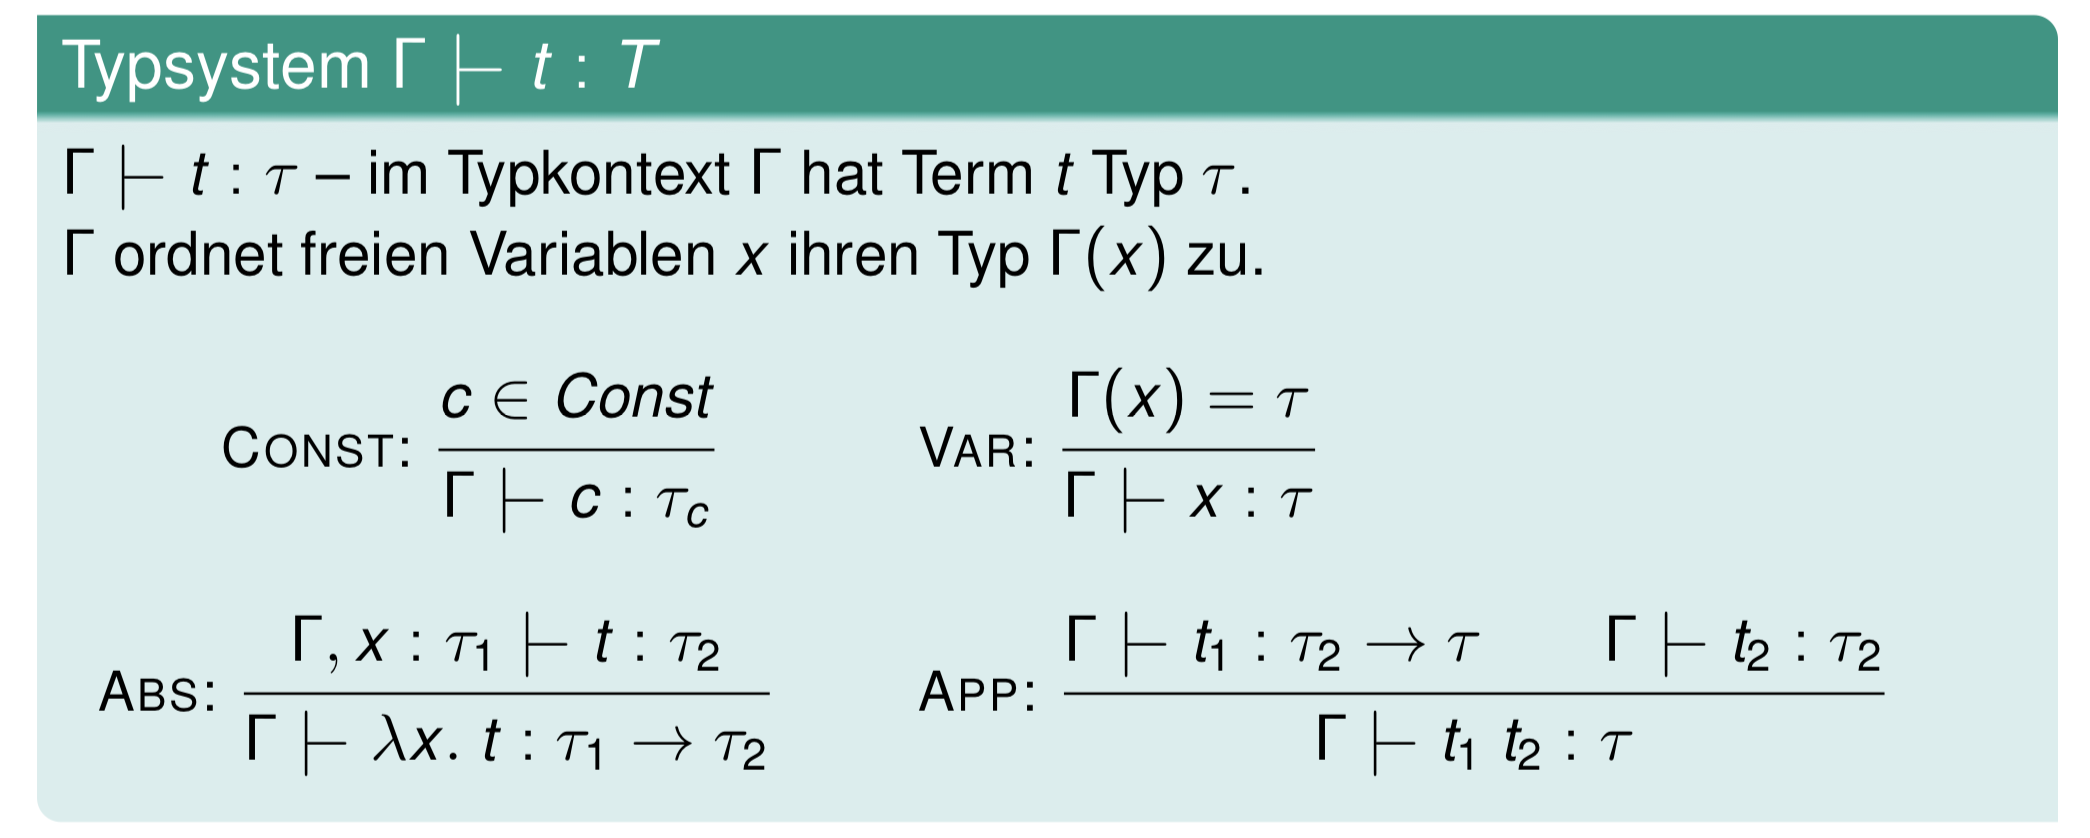
\includegraphics[width=0.75\textwidth]{images/types.png}	
\end{center}
\begin{center}
		
\includegraphics[width=0.75\textwidth]{images/let.png}
\end{center}
Beispiel:\\
\begin{center}
	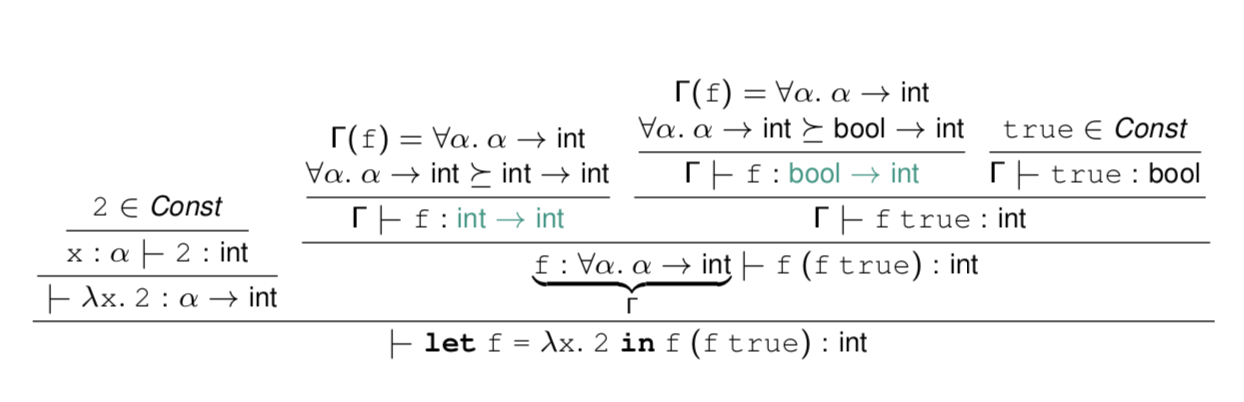
\includegraphics[width=0.75\textwidth]{images/let_ex.png}
\end{center}

